\begin{figure}[htb]
	\centering
	\begin{subfigure}{0.45\linewidth}
		\centering
		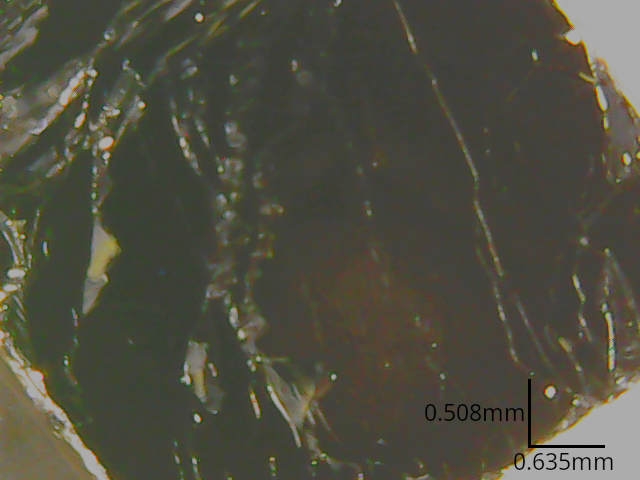
\includegraphics[width=\linewidth]{figs/hopg_skala1.png}
		\caption{Skala 1}
		\label{fig:hopg_skala1}
	\end{subfigure}
	\hspace{0.5cm}
	\begin{subfigure}{0.45\linewidth}
		\centering
		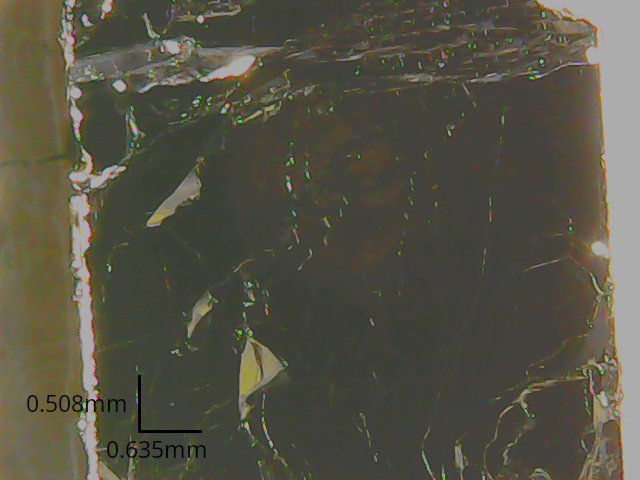
\includegraphics[width=\linewidth]{figs/hopg_skala2.png}
		\caption{Skala 2}
		\label{fig:hopg_skala2}
	\end{subfigure}
	\caption{USB-Mikroskop Aufnahmen von HOPG nach Abziehen der obersten Schicht.}
	\label{fig:usb_mikroskop_hopg}
\end{figure}